\subsubsection{\texttt{RF-5}: configuración de publicación de solución de ejercicios}
\label{subsec:rf5}

\begin{figure}[!ht]
    \centering
    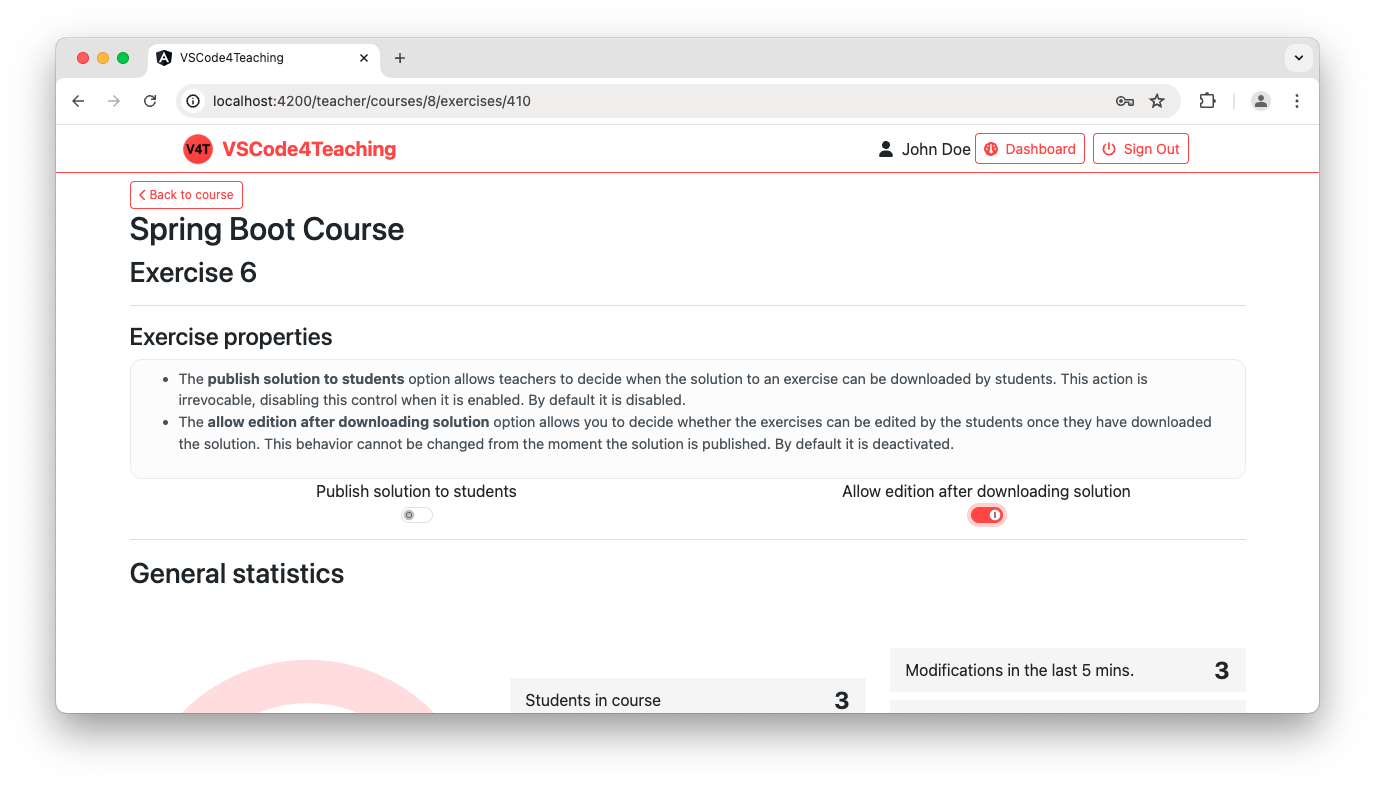
\includegraphics[width=0.9\textwidth]{imagenes/utilizadas/4-3-implementacion/rf5-1.png}
    \caption{Sección del \textit{dashboard} de los ejercicios que permite configurar los parámetros para la configuración de la disponibilidad y comportamiento de la descarga de la propuesta de solución del docente.}
    \label{fig:reqf5-1}
\end{figure}

Tal como se especifica en el requisito \referenciaConTT{subsec:rf2}{RF-2}, los ejercicios que los docentes añaden en sus cursos pueden tener asociada una propuesta de solución que los estudiantes pueden descargar en la extensión según dos parámetros de configuración de la disponibilidad de la solución que los docentes pueden ajustar en el \textit{dashboard} de cada ejercicio, tal como muestra la \referenciaFigura{fig:reqf5-1}. Los parámetros son:
\begin{itemize}
    \item \textit{Allow edition after downloading solution} (permitir edición tras descargar solución). Permite ajustar si los estudiantes pueden modificar sus propias propuestas tras descargar la solución o si, por el contrario, al descargar la propuesta de solución se deben impedir nuevas ediciones, marcándolo previamente como finalizado. Este parámetro se puede modificar mientras la solución no sea pública.
    \item \textit{Publish solution to students} (publicar solución a estudiantes). Permite configurar la disponibilidad para la descarga de la solución a los estudiantes, quienes dispondrán de un elemento gráfico en la extensión que les permitirá descargar la solución en local para, además, poder compararla mediante una interfaz gráfica para visualizar las diferencias existentes entre su propia propuesta y la solución del docente. La activación de la publicación impide la edición del parámetro anterior y, una vez publicada, esta configuración ya no puede revertirse.
\end{itemize}
